\documentclass[notes,11pt, aspectratio=169]{beamer}

\usepackage{pgfpages}
% These slides also contain speaker notes. You can print just the slides,
% just the notes, or both, depending on the setting below. Comment out the want
% you want.
\setbeameroption{hide notes} % Only slide
%\setbeameroption{show only notes} % Only notes
%\setbeameroption{show notes on second screen=right} % Both

\usepackage{helvet}
\usepackage[default]{lato}
\usepackage{array}
\usepackage{tgbonum}

\usepackage{tikz}
\usepackage{verbatim}
\setbeamertemplate{note page}{\pagecolor{yellow!5}\insertnote}
\usetikzlibrary{positioning}
\usetikzlibrary{snakes}
\usetikzlibrary{calc}
\usetikzlibrary{arrows}
\usetikzlibrary{decorations.markings}
\usetikzlibrary{shapes.misc}
\usetikzlibrary{matrix,shapes,arrows,fit,tikzmark}
\usepackage{amsmath}
\usepackage{mathpazo}
\usepackage{hyperref}
\usepackage{lipsum}
\usepackage{multimedia}
\usepackage{graphicx}
\usepackage{multirow}
\usepackage{graphicx}
\usepackage{dcolumn}
\usepackage{bbm}
\newcolumntype{d}[0]{D{.}{.}{5}}

\usepackage{changepage}
\usepackage{appendixnumberbeamer}
\newcommand{\beginbackup}{
   \newcounter{framenumbervorappendix}
   \setcounter{framenumbervorappendix}{\value{framenumber}}
   \setbeamertemplate{footline}
   {
     \leavevmode%
     \hline
     box{%
       \begin{beamercolorbox}[wd=\paperwidth,ht=2.25ex,dp=1ex,right]{footlinecolor}%
%         \insertframenumber  \hspace*{2ex} 
       \end{beamercolorbox}}%
     \vskip0pt%
   }
 }
\newcommand{\backupend}{
   \addtocounter{framenumbervorappendix}{-\value{framenumber}}
   \addtocounter{framenumber}{\value{framenumbervorappendix}} 
}


\usepackage{graphicx}
\usepackage[space]{grffile}
\usepackage{booktabs}
\newcommand\independent{\protect\mathpalette{\protect\independenT}{\perp}}
\def\independenT#1#2{\mathrel{\rlap{$#1#2$}\mkern2mu{#1#2}}}
\DeclareMathOperator{\Supp}{Supp}

% These are my colors -- there are many like them, but these ones are mine.
\definecolor{blue}{RGB}{0,114,178}
\definecolor{red}{RGB}{213,94,0}
\definecolor{yellow}{RGB}{240,228,66}
\definecolor{green}{RGB}{0,158,115}

\hypersetup{
  colorlinks=false,
  linkbordercolor = {white},
  linkcolor = {blue}
}


%% I use a beige off white for my background
\definecolor{MyBackground}{RGB}{255,253,218}

%% Uncomment this if you want to change the background color to something else
%\setbeamercolor{background canvas}{bg=MyBackground}

%% Change the bg color to adjust your transition slide background color!
\newenvironment{transitionframe}{
  \setbeamercolor{background canvas}{bg=yellow}
  \begin{frame}}{
    \end{frame}
}

\setbeamercolor{frametitle}{fg=blue}
\setbeamercolor{title}{fg=black}
\setbeamertemplate{footline}[frame number]
\setbeamertemplate{navigation symbols}{} 
\setbeamertemplate{itemize items}{-}
\setbeamercolor{itemize item}{fg=blue}
\setbeamercolor{itemize subitem}{fg=blue}
\setbeamercolor{enumerate item}{fg=blue}
\setbeamercolor{enumerate subitem}{fg=blue}
\setbeamercolor{button}{bg=MyBackground,fg=blue,}



% If you like road maps, rather than having clutter at the top, have a roadmap show up at the end of each section 
% (and after your introduction)
% Uncomment this is if you want the roadmap!
% \AtBeginSection[]
% {
%    \begin{frame}
%        \frametitle{Roadmap of Talk}
%        \tableofcontents[currentsection]
%    \end{frame}
% }
\setbeamercolor{section in toc}{fg=blue}
\setbeamercolor{subsection in toc}{fg=red}
\setbeamersize{text margin left=1em,text margin right=1em} 

\newenvironment{wideitemize}{\itemize\addtolength{\itemsep}{10pt}}{\enditemize}

\usepackage{environ}
\NewEnviron{videoframe}[1]{
  \begin{frame}
    \vspace{-8pt}
    \begin{columns}[onlytextwidth, T] % align columns
      \begin{column}{.70\textwidth}
        \begin{minipage}[t][\textheight][t]
          {\dimexpr\textwidth}
          \vspace{8pt}
          \hspace{4pt} {\Large \sc \textcolor{blue}{#1}}
          \vspace{8pt}
          
          \BODY
        \end{minipage}
      \end{column}%
      \hfill%
      \begin{column}{.38\textwidth}
        \colorbox{green!20}{\begin{minipage}[t][1.2\textheight][t]
            {\dimexpr\textwidth}
            Face goes here
          \end{minipage}}
      \end{column}%
    \end{columns}
  \end{frame}
}

\title[]{\textcolor{blue}{Canonical Research Designs I:\\ Difference-in-Differences III:\\
  }}
\author[PGP]{}
\institute[FRBNY]{\small{\begin{tabular}{c}
  Paul Goldsmith-Pinkham  \\
\end{tabular}}}

\date{\today}

\begin{document}

%%% TIKZ STUFF
\tikzset{   
        every picture/.style={remember picture,baseline},
        every node/.style={anchor=base,align=center,outer sep=1.5pt},
        every path/.style={thick},
        }
\newcommand\marktopleft[1]{%
    \tikz[overlay,remember picture] 
        \node (marker-#1-a) at (-.3em,.3em) {};%
}
\newcommand\markbottomright[2]{%
    \tikz[overlay,remember picture] 
        \node (marker-#1-b) at (0em,0em) {};%
}
\tikzstyle{every picture}+=[remember picture] 
\tikzstyle{mybox} =[draw=black, very thick, rectangle, inner sep=10pt, inner ysep=20pt]
\tikzstyle{fancytitle} =[draw=black,fill=red, text=white]
%%%% END TIKZ STUFF

% Title Slide
\begin{frame}
\maketitle
\end{frame}

\begin{frame}{Today's Topics}
  \begin{wideitemize}
  \item Complications that arise in DiD:
    \begin{enumerate}
    \item continuous treatments
    \item multiple treatments
    \item random timing
    \item Covariates + time-varying covariates
    \end{enumerate}
  \item Checklist of what you need to consider
  \end{wideitemize}
\end{frame}

\begin{frame}{Continuous treatment}
  \begin{wideitemize}
  \item Recall that estimating treatment effects with random
    assignment and continuous treatments was data hungry, but doable
  \item Without random assignment, and unconstrained heterogeneity,
    the challenge is more complicated
  \item First, consider what the estimand of interest is. Note that with potential outcomes, we now have $Y_{i}(D_{i})$ with $D_{i}$ multivalued.
  \item So what is the contrast of interest?
    \begin{align}
      ATT(d|d) &= E(Y_{i}(d) - Y_{i}(0) | D_{i} = d)\\
      ACRT(d|d) &= \frac{\partial E(Y_{i}(l) | D_{i} = d)}{\partial l}\bigg\rvert_{l = d}
    \end{align}
  \end{wideitemize}
\end{frame}

\begin{frame}{Continuous treatment -- Estimand}
  \begin{wideitemize}
  \item How do these differ? Consider their interpretations:
    \begin{itemize}
    \item ATT: effect relative to baseline of zero effect
    \item ACRT: effect of marginally increasing treatment, evaluted at a given point (can integrate too!)
    \end{itemize}
  \item Key point in DiD vs. RCT: these are \emph{conditional} on treatment status, which is not random!
  \item Can we move between these? Consider comparing two ATTs in 2
    period diff-in-diff, assuming standard parallel trends:
    \begin{align*}
      ATT(d | d) -  ATT(d' | d') &= \left(E[\Delta Y | D = d]  - E[\Delta Y | D=0]\right)\\
                                 &- \left(E[\Delta Y | D = d']  - E[\Delta Y | D=0]\right)\\
                                 &= E[\Delta Y | D = d]  - E[\Delta Y | D = d']\\
                                 &= E[\Delta Y(d) - \Delta Y(d') | D = d]  + ATT(d' | d) - ATT(d' | d')
    \end{align*}
  \end{wideitemize}
\end{frame}

\begin{frame}{Continuous treatment -- challenge}
  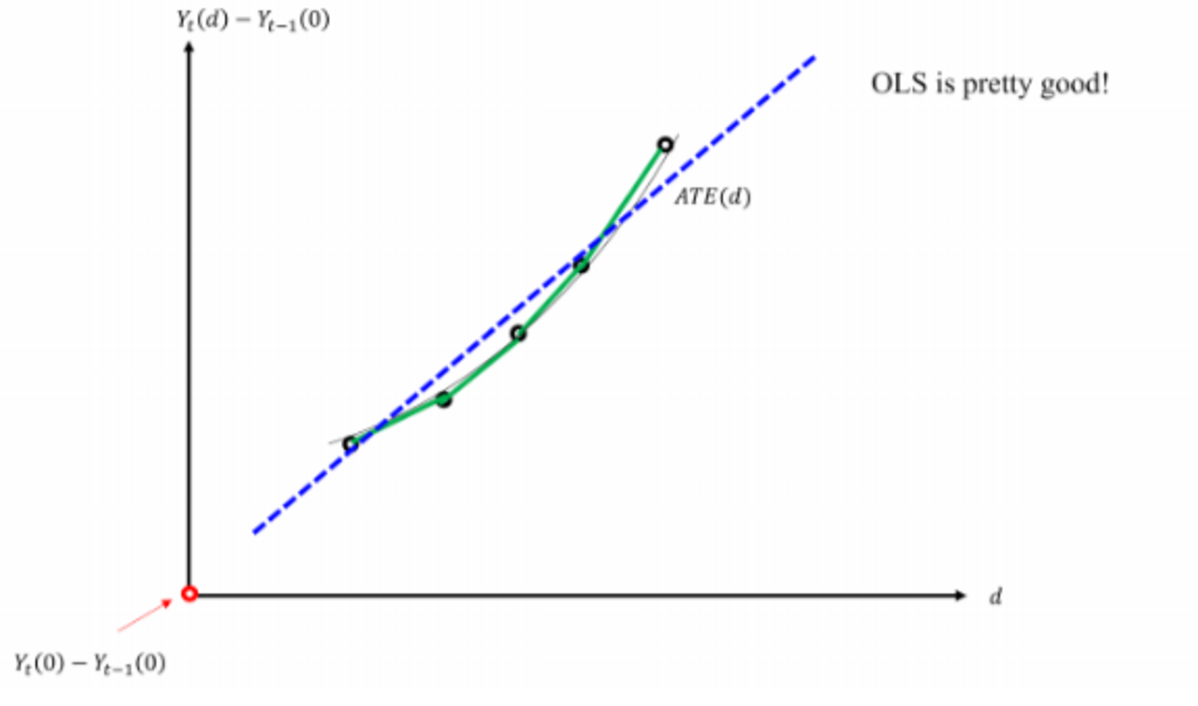
\includegraphics[width=0.8\linewidth]{images/continuous_did_1.pdf}
\end{frame}

\begin{frame}{Continuous treatment -- challenge}
  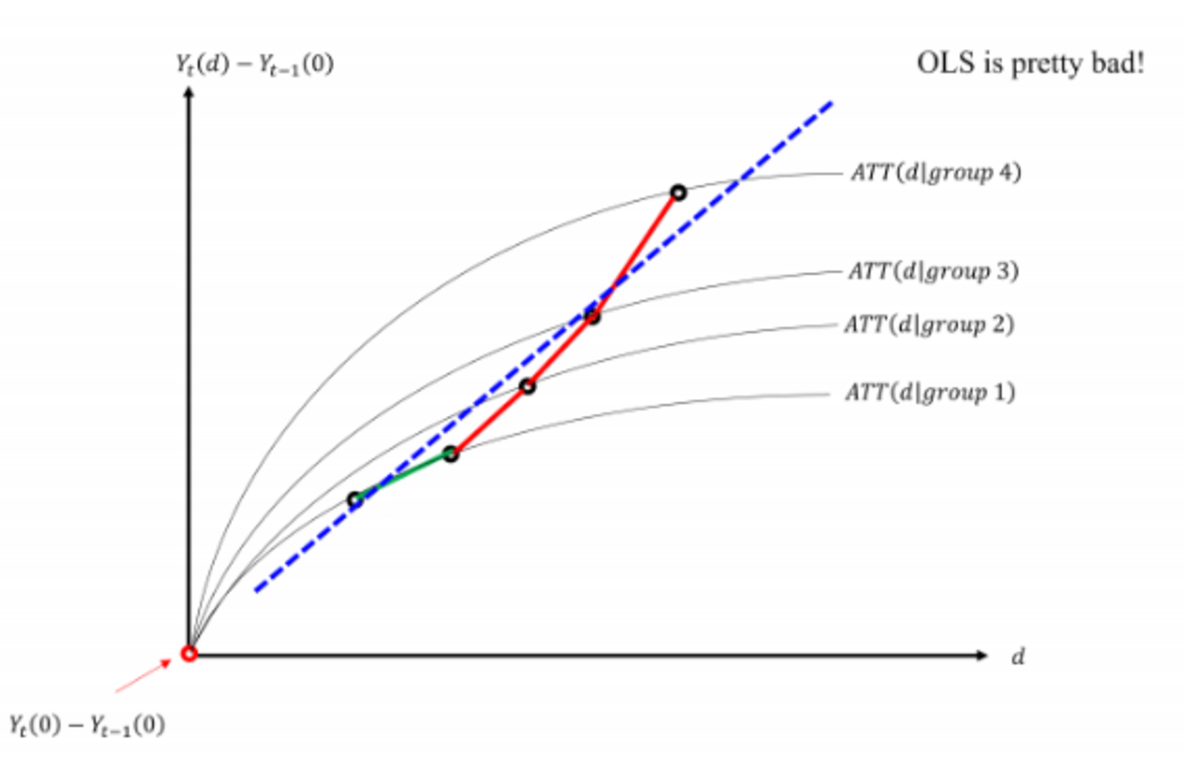
\includegraphics[width=0.8\linewidth]{images/continuous_did_2.pdf}
\end{frame}

\begin{frame}{Continuous treatment -- stronger assumption about heterogeneity}
  \begin{wideitemize}
  \item ``Strong'' parallel trends assumption: $E(\Delta Y_{i}(d)) = E(\Delta Y_{i}(d) | D_{i} = d)$
  \item No selection bias ``on average''
  \item Effectively assuming some kind of homogeneity in the treatment across groups
  \end{wideitemize}
\end{frame}

\begin{frame}{Multiple Treatments in Diff-in-diff}
  \begin{wideitemize}
  \item Hull (2018) and deChaisemartin and D'hautefeuille (2022) are relevant cites
  \item One ``easy'' context that this shows up (Hull 2018) is ``mover'' designs
    \begin{itemize}
    \item I move from city $i$ to city $j$ -- if my move was random,
      can we use it to understand the effect of city $j$?
    \item Without strong additional assumptions, challenging to
      interpret coefficients from standard TWFE
      \begin{equation}
        Y_{it} = \alpha_{i} + \tau_{t} + \sum_{j\not=0}\beta_{j}D_{ijt} + \epsilon_{it}
      \end{equation}
    \end{itemize}
  \item Consider 2 period case, and use first differences:
    \begin{equation}
      \Delta Y_{i} = \tau + \sum_{j\not=0}\beta_{j}\Delta D_{ij} + \Delta\epsilon_{i}          
    \end{equation}
  \item Recall Goldsmith-Pinkham, Hull and Kolesar (2022) -- multiple
    treatments ($\Delta D_{ij}$) is potentially contaminated and
    negative weighted.
  \end{wideitemize}
\end{frame}


\begin{frame}{Random Timing in Diff-in-Diff}
  \begin{wideitemize}
  \item Athey and Imbens (2022) take design-based approach to diff-in-diff
    \begin{itemize}
    \item What does this mean? Can consider a well-defined propensity scores for the treatment
    \item Focus on staggered adoption with binary treatment
    \item Since treamtent is absorbing, this simplifies problem into ``when did I get the treatment (if ever)?''
    \end{itemize}
  \item E.g. define a propensity score: $Pr(A_{i} = a)$ over when the assignment occurs.
  \item Key question: who is the relevant counterfactual group?
  \end{wideitemize}
\end{frame}

\begin{frame}{Three key assumptions (not testable!)}
  \begin{enumerate}
  \item Random assignment (can make this happen by design)
  \item No anticipation (we assume this already)
  \item Invariance to history
    ($1_{a \leq t}(Y_{it}(a) - Y_{it}(1)) = 0$) (no causal effect of
    an early adotpion vs. a later adoption on outcome as long as
    adoption occured before or on period $t$)
  \end{enumerate}
\end{frame}

\begin{frame}{Efficiency in estimating staggered random roll-out}
  \begin{wideitemize}
  \item Roth and Sant'anna (2023) show that it is much more efficient
    to condition on lagged outcomes over using standard diff-in-diff
    in staggered roll-outs
  \item E.g. Consider the class of estimators:
    \begin{equation}
      \hat{\theta}_{\beta} = (\overline{Y}_{22} - \overline{Y}_{2\infty}) -  \beta(\overline{Y}_{12} - \overline{Y}_{1\infty})
    \end{equation}
    Did is the special case of $\beta=1$.
  \item We want to put more weight on this setting when the lagged
    outcomes are more predictive, and less when it is not!
    \begin{itemize}
    \item Intuition is similar to synthetic controls
    \end{itemize}
  \end{wideitemize}
\end{frame}

\begin{frame}{Covariates}
  \begin{wideitemize}
  \item With time-invariant covariates that treatment does not affect,
    controlling for covariates is conditional parallel trends
    assumption
    \begin{equation}
      E(Y_{i,2}(0)-Y_{i,1}(0) | D_{i} = 1, X_{i}) =       E(Y_{i,2}(0)-Y_{i,1}(0) | D_{i} = 0, X_{i})
    \end{equation}
  \item However, this isn't enough to satisfy this TWFE regression approach in two periods:
    \begin{equation}
      Y_{it} = \alpha_{i} + \phi_{t} + 1(t=2)D_{i}\beta + X_{i}1(t = 2)\gamma + \epsilon_{it}
    \end{equation}
    Why? (consider age)
  \item Even worse, if covariates affected by treatment, this is a form of
    collider bias!
    \begin{itemize}
    \item Should be very careful about time-varying covariates
    \end{itemize}
  \end{wideitemize}
\end{frame}


\begin{frame}{Checklist}
  \begin{wideitemize}
  \item First, consider the treatment features of your setup
      \begin{itemize}
    \item What is your treatment? Binary or continuous?
    \item Single or multiple?
    \item Absorbing or not?
    \item How many treated units? Single or many?
    \item How many interventions? Single or staggered timing?
    \end{itemize}
  \item Second, consider the relevant identifying assumptions for your condition
  \item Third, what tests are feasible in your setting?
  \item Fourth, what estimates do you want?
  \item Fifth, what relaxations of assumptions can you make?
  \end{wideitemize}
\end{frame}

\begin{frame}{Treatment features}
  \begin{wideitemize}
  \item If treatment is binary or only a few values, easy to consider the simple case
    \begin{itemize}
    \item Particularly helps if it's absorbing!
    \end{itemize}
  \item If continuous and/or not absorbing, need to worry about many more homogeneity assumptions
  \item First order of business -- \emph{define your estimand}.
    \begin{itemize}
    \item What treatment do you care about?
    \end{itemize}
  \item Can you simplify the problem in some way if it's more complex?
  \end{wideitemize}
\end{frame}

\begin{frame}{Assumptions}
  \begin{wideitemize}
  \item Write out carefully in math and then words what assumptions you need
    \begin{itemize}
    \item Parallel trends (with or without covariates)?
    \item No anticipation?
    \item Others?
    \end{itemize}
  \item If you know your estimand, much easier to know what you need
  \item Do you need to construct your estimator using lagged outcomes, e.g. synthetic control? 
  \end{wideitemize}
\end{frame}

\begin{frame}{Testable assumptions}
  \begin{wideitemize}
  \item What is testable? Pre-trends can be useful, but underpowered
  \item If using random timing, not much is testable
    \begin{itemize}
    \item But could look for balance across timing groups in exogeneous features
    \end{itemize}
  \end{wideitemize}
\end{frame}

\begin{frame}{What estimates do you want?}
  \begin{wideitemize}
  \item Do you need a long run effect? Short-run?
    \begin{itemize}
    \item Long-run effect relies \emph{heavily} on parametric
      extrapolation. Is it plausible?
    \end{itemize}
  \item Are you studying ATTs? CATTs? ACRTs?
  \end{wideitemize}
\end{frame}

\begin{frame}{Relaxation of assumptions?}
  \begin{wideitemize}
  \item What group comparaisons are you making for parallel trends?
  \item Could you assume random timing instead of parallel trends?
  \item Could you condition on lagged outcomes?
  \end{wideitemize}
\end{frame}
\end{document}